%%% One-side print:
\documentclass[11pt,a4paper]{report}
\usepackage[top=25mm,bottom=25mm,right=25mm,left=30mm,head=12.5mm,foot=12.5mm]{geometry}
\let\openright=\clearpage

%%% Two-side print:
%\documentclass[11pt,a4paper,twoside,openright]{report}
%\usepackage[top=25mm,bottom=25mm,right=25mm,left=30mm,head=12.5mm,foot=12.5mm]{geometry}
%\let\openright=\cleardoublepage

%%% Definition of some useful macros
%%% Tento soubor obsahuje definice různých užitečných maker a prostředí %%%
%%% Další makra připisujte sem, ať nepřekáží v ostatních souborech.     %%%
%%% This file contains definitions of various useful macros and environments      %%%
%%% Assign additional macros here so that they do not interfere with other files. %%%

\usepackage[a-2u]{pdfx}     % výsledné PDF bude ve standardu PDF/A-2u
                            % resulting PDF will be in the PDF / A-2u standard

\usepackage{ifpdf}
\usepackage{ifxetex}
\usepackage{ifluatex}

%%% Nastavení pro použití samostatné bibliografické databáze.
%%% Settings for using a separate bibliographic database.
\usepackage[
   backend=biber
 ,style=iso-authoryear
  % ,style=iso-numeric
  ,sortlocale=cs_CZ
  ,alldates=iso
  ,bibencoding=UTF8
  ,maxnames=2
  ,maxbibnames=99
  ,block=ragged
]{biblatex}
\let\cite\parencite
\renewcommand*{\multinamedelim}{, \addspace}
\renewcommand*{\finalnamedelim}{\addspace a \addspace}

\bibliography{bibliography}

%% Přepneme na českou sazbu, fonty Latin Modern a kódování češtiny
\ifthenelse{\boolean{xetex}\OR\boolean{luatex}}
   { % use fontspec and OpenType fonts with utf8 engines
			\usepackage[english,slovak,czech]{babel}
			\usepackage[autostyle,english=british,czech=quotes]{csquotes}
			\usepackage{fontspec}
			\defaultfontfeatures{Ligatures=TeX,Scale=MatchLowercase}
   }
   {
			\usepackage[english,slovak,czech]{babel}
			\usepackage{lmodern}
			\usepackage[T1]{fontenc}
			\usepackage{textcomp}
			\usepackage[utf8]{inputenc}
			\usepackage[autostyle,english=british,czech=quotes]{csquotes}
	 }
\ifluatex
\makeatletter
\let\pdfstrcmp\pdf@strcmp
\makeatother
\fi

%%% Další užitečné balíčky (jsou součástí běžných distribucí LaTeXu)
\usepackage{amsmath}        % rozšíření pro sazbu matematiky / extension for math typesetting
\usepackage{amsfonts}       % matematické fonty / mathematical fonts
\usepackage{amssymb}        % symboly / symbols
\usepackage{amsthm}         % sazba vět, definic apod. / typesetting of sentences, definitions, etc.
\usepackage{bm}             % tučné symboly (příkaz \bm) / bold symbols (\bm command)
\usepackage{graphicx}       % vkládání obrázků / graphics inserting
\usepackage{listings}       % vylepšené prostředí pro strojové písmo / improved environment for source codes typesetting
\usepackage{fancyhdr}       % prostředí pohodlnější nastavení hlavy a paty stránek / environment for more comfortable adjustment of the head and foot of the pages
\usepackage{icomma}         % inteligetní čárka v matematickém módu / intelligent comma in math mode
\usepackage{dcolumn}        % lepší zarovnání sloupců v tabulkách / better alignment of columns in tables
\usepackage{booktabs}       % lepší vodorovné linky v tabulkách / better horizontal lines in tables
\makeatletter
\@ifpackageloaded{xcolor}{
   \@ifpackagewith{xcolor}{usenames}{}{\PassOptionsToPackage{usenames}{xcolor}}
  }{\usepackage[usenames]{xcolor}} % barevná sazba / color typesetting
\makeatother
\usepackage{multicol}       % práce s více sloupci na stránce / work with multiple columns on a page
\usepackage{caption}
\usepackage{enumitem}
\setlist[itemize]{noitemsep, topsep=0pt, partopsep=0pt}
\setlist[enumerate]{noitemsep, topsep=0pt, partopsep=0pt}
\setlist[description]{noitemsep, topsep=0pt, partopsep=0pt}

\usepackage{tocloft}
\setlength\cftparskip{0pt}
\setlength\cftbeforechapskip{1.5ex}
\setlength\cftfigindent{0pt}
\setlength\cfttabindent{0pt}
\setlength\cftbeforeloftitleskip{0pt}
\setlength\cftbeforelottitleskip{0pt}
\setlength\cftbeforetoctitleskip{0pt}
\renewcommand{\cftlottitlefont}{\Huge\bfseries\sffamily}
\renewcommand{\cftloftitlefont}{\Huge\bfseries\sffamily}
\renewcommand{\cfttoctitlefont}{\Huge\bfseries\sffamily}

% vyznaceni odstavcu
% differentiation of new paragraphs
\parindent=0pt
\parskip=11pt

% zakaz vdov a sirotku - jednoradkovych pocatku ci koncu odstavcu na prechodu mezi strankami
% Prohibition of widows and orphans - single-line beginning and end of paragraph at the transition between pages
\clubpenalty=1000
\widowpenalty=1000
\displaywidowpenalty=1000

% nastaveni radkovani
% setting of line spacing
\renewcommand{\baselinestretch}{1.20}

% nastaveni pro nadpisy - tucne a bezpatkove
% settings for headings - bold and sans serif
\usepackage{sectsty}    
\allsectionsfont{\sffamily}

% nastavení hlavy a paty stránek
% page head and foot settings
\makeatletter
\if@twoside%
    \fancypagestyle{fancyx}{%
			\fancyhf{}                                     
      \fancyhead[RE]{\rightmark}                  
      \fancyhead[LO]{\leftmark}                  
      \fancyfoot[RO,LE]{\thepage}                    
      \renewcommand{\headrulewidth}{.5pt}            
      \renewcommand{\footrulewidth}{.5pt}            
    }
    \fancypagestyle{plain}{%
			\fancyhf{}                                     
    	\fancyfoot[RO,LE]{\thepage}                    
    	\renewcommand{\headrulewidth}{0pt}             
    	\renewcommand{\footrulewidth}{0.5pt}
    }          
\else
    \fancypagestyle{fancyx}{%
			\fancyhf{}                                     
      \fancyhead[R]{\leftmark}                  
      \fancyfoot[R]{\thepage}                    
      \renewcommand{\headrulewidth}{.5pt}            
      \renewcommand{\footrulewidth}{.5pt}            
    }
    \fancypagestyle{plain}{%                       
    	\fancyhf{} % clear all header and footer fields
    	\fancyfoot[R]{\thepage}                    
    	\renewcommand{\headrulewidth}{0pt}             
    	\renewcommand{\footrulewidth}{0.5pt}
    }          
\fi
\renewcommand*{\cleardoublepage}{\clearpage\if@twoside \ifodd\c@page\else
	\hbox{}%
	\thispagestyle{empty}%
	\newpage%
	\if@twocolumn\hbox{}\newpage\fi\fi\fi
}
\makeatother

% Tato makra přesvědčují mírně ošklivým trikem LaTeX, aby hlavičky kapitol
% sázel příčetněji a nevynechával nad nimi spoustu místa. Směle ignorujte.
% These macros convince with a slightly ugly LaTeX trick to make chapter headers
% bet more sane and didn't miss a lot of space above them. Be boldly ignore it.
\makeatletter
\def\@makechapterhead#1{
  {\parindent \z@ \raggedright \sffamily
   \Huge\bfseries \thechapter. #1
   \par\nobreak
   \vskip 20\p@
}}
\def\@makeschapterhead#1{
  {\parindent \z@ \raggedright \sffamily
   \Huge\bfseries #1
   \par\nobreak
   \vskip 20\p@
}}
\makeatother

% Trochu volnější nastavení dělení slov, než je default.
% Slightly looser hyphenation setting than default.
\lefthyphenmin=2
\righthyphenmin=2

% Zapne černé "slimáky" na koncích řádků, které přetekly, abychom si jich lépe všimli.
% Turns on the black "snails" at the ends of the lines that overflowed to get us noticed them better.
% \overfullrule=1mm

%% Balíček hyperref, kterým jdou vyrábět klikací odkazy v PDF,
%% ale hlavně ho používáme k uložení metadat do PDF (včetně obsahu).
%% Většinu nastavítek přednastaví balíček pdfx.
%% A hyperref package that can be used to produce clickable links in PDF,
%% but we mainly use it to store metadata in PDF (including content).
%% Most settings are preset by the pdfx package.
\hypersetup{unicode}
\hypersetup{breaklinks=true}
\hypersetup{hidelinks}

% Přejmenování objektů autoref pro odkazování v textu
\renewcommand{\chapterautorefname}{Kapitola}
\renewcommand{\sectionautorefname}{Sekce}
\renewcommand{\subsectionautorefname}{Podsekce}
\renewcommand{\tableautorefname}{Tabulka}
\renewcommand{\figureautorefname}{Obrázek}
\renewcommand{\equationautorefname}{Rovnice}



\renewcommand{\UrlBreaks}{\do\/\do\=\do\+\do\-\do\_\do\ \do\a\do\b\do\c\do\d%
\do\e\do\f\do\g\do\h\do\i\do\j\do\k\do\l\do\m\do\n\do\o\do\p\do\q\do\r\do\s%
\do\t\do\u\do\v\do\w\do\x\do\y\do\z\do\A\do\B\do\C\do\D\do\E\do\F\do\G\do\H%
\do\I\do\J\do\K\do\L\do\M\do\N\do\O\do\P\do\Q\do\R\do\S\do\T\do\U\do\V\do\W%
\do\X\do\Y\do\Z\do\1\do\2\do\3\do\4\do\5\do\6\do\7\do\8\do\9\do\0}

\renewcommand{\mid}{|}

%%% Prostředí pro sazbu kódu, případně vstupu/výstupu počítačových
%%% programů. (Vyžaduje balíček listings -- fancy verbatim.)
%%% Environment for source code typesetting, or computer input/output
%%% programs. (Requires package listings - fancy verbatim.)
\lstnewenvironment{code}{\lstset{basicstyle=\small, frame=single}}{}

%%% User-defined balíčky
\usepackage{dsfont}

\theoremstyle{definition}
\newtheorem{definition}{Definice}[section]
\newcommand{\definitionautorefname}{Definice}

\usepackage{float}
\usepackage{tikz}
\usetikzlibrary{fit,arrows.meta,automata,positioning,shapes.geometric,trees}

\usepackage{tikzscale}

\usepackage{forest}

\usepackage[ruled]{algorithm2e}
\usepackage{subfig}
\usepackage{pdflscape}
\usepackage{minted}

\usepackage{neuralnetwork}
\newcommand{\xin}[2]{$x_#2$}
\newcommand{\xout}[2]{$\hat x_#2$}

\DeclareMathOperator{\tr}{\text{tr}}
\SetAlgorithmName{Algoritmus}{Algoritmus}




%%% DEFINITION OF BASIC VARIABLES
\def\TypPrace{BP}                % bakalářská práce/bachelor thesis
%\def\TypPrace{DP}               % diplomová práce/master thesis
\def\Jazyk{cze}                  % čeština/czech
%\def\Jazyk{slo}                 % slovenština/slovak
%\def\Jazyk{eng}                 % angličtina/english

%%% Název práce v jazyce práce (přesně podle zadání)
%%% Title of the thesis in the language used in the text (exact according to assignment)
\def\NazevPrace{Variační autoenkodér a úlohy pozorování v latentním prostoru}

%%% Tento soubor obsahuje definice různých užitečných maker a prostředí %%%
%%% Další makra připisujte sem, ať nepřekáží v ostatních souborech.     %%%
%%% This file contains definitions of various useful macros and environments      %%%
%%% Assign additional macros here so that they do not interfere with other files. %%%

\usepackage[a-2u]{pdfx}     % výsledné PDF bude ve standardu PDF/A-2u
                            % resulting PDF will be in the PDF / A-2u standard

\usepackage{ifpdf}
\usepackage{ifxetex}
\usepackage{ifluatex}

%%% Nastavení pro použití samostatné bibliografické databáze.
%%% Settings for using a separate bibliographic database.
\usepackage[
   backend=biber
 ,style=iso-authoryear
  % ,style=iso-numeric
  ,sortlocale=cs_CZ
  ,alldates=iso
  ,bibencoding=UTF8
  ,maxnames=2
  ,maxbibnames=99
  ,block=ragged
]{biblatex}
\let\cite\parencite
\renewcommand*{\multinamedelim}{, \addspace}
\renewcommand*{\finalnamedelim}{\addspace a \addspace}

\bibliography{bibliography}

%% Přepneme na českou sazbu, fonty Latin Modern a kódování češtiny
\ifthenelse{\boolean{xetex}\OR\boolean{luatex}}
   { % use fontspec and OpenType fonts with utf8 engines
			\usepackage[english,slovak,czech]{babel}
			\usepackage[autostyle,english=british,czech=quotes]{csquotes}
			\usepackage{fontspec}
			\defaultfontfeatures{Ligatures=TeX,Scale=MatchLowercase}
   }
   {
			\usepackage[english,slovak,czech]{babel}
			\usepackage{lmodern}
			\usepackage[T1]{fontenc}
			\usepackage{textcomp}
			\usepackage[utf8]{inputenc}
			\usepackage[autostyle,english=british,czech=quotes]{csquotes}
	 }
\ifluatex
\makeatletter
\let\pdfstrcmp\pdf@strcmp
\makeatother
\fi

%%% Další užitečné balíčky (jsou součástí běžných distribucí LaTeXu)
\usepackage{amsmath}        % rozšíření pro sazbu matematiky / extension for math typesetting
\usepackage{amsfonts}       % matematické fonty / mathematical fonts
\usepackage{amssymb}        % symboly / symbols
\usepackage{amsthm}         % sazba vět, definic apod. / typesetting of sentences, definitions, etc.
\usepackage{bm}             % tučné symboly (příkaz \bm) / bold symbols (\bm command)
\usepackage{graphicx}       % vkládání obrázků / graphics inserting
\usepackage{listings}       % vylepšené prostředí pro strojové písmo / improved environment for source codes typesetting
\usepackage{fancyhdr}       % prostředí pohodlnější nastavení hlavy a paty stránek / environment for more comfortable adjustment of the head and foot of the pages
\usepackage{icomma}         % inteligetní čárka v matematickém módu / intelligent comma in math mode
\usepackage{dcolumn}        % lepší zarovnání sloupců v tabulkách / better alignment of columns in tables
\usepackage{booktabs}       % lepší vodorovné linky v tabulkách / better horizontal lines in tables
\makeatletter
\@ifpackageloaded{xcolor}{
   \@ifpackagewith{xcolor}{usenames}{}{\PassOptionsToPackage{usenames}{xcolor}}
  }{\usepackage[usenames]{xcolor}} % barevná sazba / color typesetting
\makeatother
\usepackage{multicol}       % práce s více sloupci na stránce / work with multiple columns on a page
\usepackage{caption}
\usepackage{enumitem}
\setlist[itemize]{noitemsep, topsep=0pt, partopsep=0pt}
\setlist[enumerate]{noitemsep, topsep=0pt, partopsep=0pt}
\setlist[description]{noitemsep, topsep=0pt, partopsep=0pt}

\usepackage{tocloft}
\setlength\cftparskip{0pt}
\setlength\cftbeforechapskip{1.5ex}
\setlength\cftfigindent{0pt}
\setlength\cfttabindent{0pt}
\setlength\cftbeforeloftitleskip{0pt}
\setlength\cftbeforelottitleskip{0pt}
\setlength\cftbeforetoctitleskip{0pt}
\renewcommand{\cftlottitlefont}{\Huge\bfseries\sffamily}
\renewcommand{\cftloftitlefont}{\Huge\bfseries\sffamily}
\renewcommand{\cfttoctitlefont}{\Huge\bfseries\sffamily}

% vyznaceni odstavcu
% differentiation of new paragraphs
\parindent=0pt
\parskip=11pt

% zakaz vdov a sirotku - jednoradkovych pocatku ci koncu odstavcu na prechodu mezi strankami
% Prohibition of widows and orphans - single-line beginning and end of paragraph at the transition between pages
\clubpenalty=1000
\widowpenalty=1000
\displaywidowpenalty=1000

% nastaveni radkovani
% setting of line spacing
\renewcommand{\baselinestretch}{1.20}

% nastaveni pro nadpisy - tucne a bezpatkove
% settings for headings - bold and sans serif
\usepackage{sectsty}    
\allsectionsfont{\sffamily}

% nastavení hlavy a paty stránek
% page head and foot settings
\makeatletter
\if@twoside%
    \fancypagestyle{fancyx}{%
			\fancyhf{}                                     
      \fancyhead[RE]{\rightmark}                  
      \fancyhead[LO]{\leftmark}                  
      \fancyfoot[RO,LE]{\thepage}                    
      \renewcommand{\headrulewidth}{.5pt}            
      \renewcommand{\footrulewidth}{.5pt}            
    }
    \fancypagestyle{plain}{%
			\fancyhf{}                                     
    	\fancyfoot[RO,LE]{\thepage}                    
    	\renewcommand{\headrulewidth}{0pt}             
    	\renewcommand{\footrulewidth}{0.5pt}
    }          
\else
    \fancypagestyle{fancyx}{%
			\fancyhf{}                                     
      \fancyhead[R]{\leftmark}                  
      \fancyfoot[R]{\thepage}                    
      \renewcommand{\headrulewidth}{.5pt}            
      \renewcommand{\footrulewidth}{.5pt}            
    }
    \fancypagestyle{plain}{%                       
    	\fancyhf{} % clear all header and footer fields
    	\fancyfoot[R]{\thepage}                    
    	\renewcommand{\headrulewidth}{0pt}             
    	\renewcommand{\footrulewidth}{0.5pt}
    }          
\fi
\renewcommand*{\cleardoublepage}{\clearpage\if@twoside \ifodd\c@page\else
	\hbox{}%
	\thispagestyle{empty}%
	\newpage%
	\if@twocolumn\hbox{}\newpage\fi\fi\fi
}
\makeatother

% Tato makra přesvědčují mírně ošklivým trikem LaTeX, aby hlavičky kapitol
% sázel příčetněji a nevynechával nad nimi spoustu místa. Směle ignorujte.
% These macros convince with a slightly ugly LaTeX trick to make chapter headers
% bet more sane and didn't miss a lot of space above them. Be boldly ignore it.
\makeatletter
\def\@makechapterhead#1{
  {\parindent \z@ \raggedright \sffamily
   \Huge\bfseries \thechapter. #1
   \par\nobreak
   \vskip 20\p@
}}
\def\@makeschapterhead#1{
  {\parindent \z@ \raggedright \sffamily
   \Huge\bfseries #1
   \par\nobreak
   \vskip 20\p@
}}
\makeatother

% Trochu volnější nastavení dělení slov, než je default.
% Slightly looser hyphenation setting than default.
\lefthyphenmin=2
\righthyphenmin=2

% Zapne černé "slimáky" na koncích řádků, které přetekly, abychom si jich lépe všimli.
% Turns on the black "snails" at the ends of the lines that overflowed to get us noticed them better.
% \overfullrule=1mm

%% Balíček hyperref, kterým jdou vyrábět klikací odkazy v PDF,
%% ale hlavně ho používáme k uložení metadat do PDF (včetně obsahu).
%% Většinu nastavítek přednastaví balíček pdfx.
%% A hyperref package that can be used to produce clickable links in PDF,
%% but we mainly use it to store metadata in PDF (including content).
%% Most settings are preset by the pdfx package.
\hypersetup{unicode}
\hypersetup{breaklinks=true}
\hypersetup{hidelinks}

% Přejmenování objektů autoref pro odkazování v textu
\renewcommand{\chapterautorefname}{Kapitola}
\renewcommand{\sectionautorefname}{Sekce}
\renewcommand{\subsectionautorefname}{Podsekce}
\renewcommand{\tableautorefname}{Tabulka}
\renewcommand{\figureautorefname}{Obrázek}
\renewcommand{\equationautorefname}{Rovnice}



\renewcommand{\UrlBreaks}{\do\/\do\=\do\+\do\-\do\_\do\ \do\a\do\b\do\c\do\d%
\do\e\do\f\do\g\do\h\do\i\do\j\do\k\do\l\do\m\do\n\do\o\do\p\do\q\do\r\do\s%
\do\t\do\u\do\v\do\w\do\x\do\y\do\z\do\A\do\B\do\C\do\D\do\E\do\F\do\G\do\H%
\do\I\do\J\do\K\do\L\do\M\do\N\do\O\do\P\do\Q\do\R\do\S\do\T\do\U\do\V\do\W%
\do\X\do\Y\do\Z\do\1\do\2\do\3\do\4\do\5\do\6\do\7\do\8\do\9\do\0}

\renewcommand{\mid}{|}

%%% Prostředí pro sazbu kódu, případně vstupu/výstupu počítačových
%%% programů. (Vyžaduje balíček listings -- fancy verbatim.)
%%% Environment for source code typesetting, or computer input/output
%%% programs. (Requires package listings - fancy verbatim.)
\lstnewenvironment{code}{\lstset{basicstyle=\small, frame=single}}{}

%%% User-defined balíčky
\usepackage{dsfont}

\theoremstyle{definition}
\newtheorem{definition}{Definice}[section]
\newcommand{\definitionautorefname}{Definice}

\usepackage{float}
\usepackage{tikz}
\usetikzlibrary{fit,arrows.meta,automata,positioning,shapes.geometric,trees}

\usepackage{tikzscale}

\usepackage{forest}

\usepackage[ruled]{algorithm2e}
\usepackage{subfig}
\usepackage{pdflscape}
\usepackage{minted}

\usepackage{neuralnetwork}
\newcommand{\xin}[2]{$x_#2$}
\newcommand{\xout}[2]{$\hat x_#2$}

\DeclareMathOperator{\tr}{\text{tr}}
\SetAlgorithmName{Algoritmus}{Algoritmus}




%%% Jméno autora
%%% Author's name - First name Surname
\def\AutorPrace{Tomáš Faltejsek}

%%% Rok odevzdání a měsíc (slovně)
%%% Year of submission and month (verbally) - month YYYY
\def\DatumOdevzdani{květen 2023}

%%% Vedoucí práce: Jméno a příjmení s~tituly
%%% Supervisor: First name and surname with titles
\def\Vedouci{Ing. Ondřej Vadinský, Ph.D.}

%%% Konzultant práce: Jméno a příjmení s~tituly
%%% Consultant: First name and surname with titles
\def\Konzultant{full consultant’s name (incl. degrees)}

%%% Studijní program
%%% Study program
\def\StudijniProgram{Aplikovaná informatika}

%%% Studijní program - specializace
%%% Study program - specialization
\def\Specializace{}

%%% Studijní obor
%%% Field of study
\def\StudijniObor{Aplikovaná informatika}

%%% Nepovinné poděkování (vedoucímu práce, konzultantovi, tomu, kdo zapůjčil software, literaturu apod.)
%%% Optional thanks (the supervisor, the consultant, the borrower of software, literature, etc.)
\def\Podekovani{%
Thanks.
}

%%% Abstract (recommended range of about 150-250 words; this is not a thesis assignment)
\def\Abstrakt{%
Jedním z předních rysů lidské inteligence je intuice a schopnost představovat si nové objekty. Variační autoenkodér je inovací na poli pravděpodobnostních modelů, umožňující architekturu modelů schopných syntézy zcela nových dat s využitím pozorování atributů v latentním prostoru. Teoretická charakteristika a možnosti využití variačního autoenkodéru jsou předmětem této bakalářské práce.
}
\def\KlicovaSlova{keyword, important term, another topic, and another one}


%%% Titulní strana a různé povinné informativní strany
%%% Title page and various mandatory information pages
\begin{document}
%%% Titulní strana práce a další povinné informační strany
%%% Title page of the thesis and other obligatory information pages

%%% Titulní strana práce
%%% Title page of the thesis

\pagestyle{empty}
\hypersetup{pageanchor=false}

\begin{center}
\Huge\sffamily
\VSE\\
\FIS

\vspace{\stretch{1}}

\ifstringequal{\Jazyk}{eng}{
	
\includegraphics[width=.5\textwidth]{img/FIS_2_logo_2_rgb_EN}
}{
	
\includegraphics[width=.5\textwidth]{img/FIS_2_logo_2_rgb_EN}
	% 
\includegraphics[width=.5\textwidth]{img/FIS_2_logo_2_rgb_CZ} TODO: Add CZ variant of the logo
}

\vspace{\stretch{2}}

\bfseries\NazevPrace

\vspace{8mm}
\mdseries\TypPraceText

\vspace{8mm}
\large
\begin{tabular}{rl}
\StudijniProgramText: & \StudijniProgram \\
\ifthenelse{\equal{\Specializace}{}}{%
	% empty value
	}{
	\rule{0pt}{6mm}%
	\SpecializaceText: & \Specializace \\
}
\ifthenelse{\equal{\StudijniObor}{}}{%
	% empty value
	}{
	\rule{0pt}{6mm}%
	\StudijniOborText: & \StudijniObor \\
}
\end{tabular}

\vspace{\stretch{8}}

\begin{tabular}{rl}
\AutorText: & \AutorPrace \\
\noalign{\vspace{2mm}}
\VedouciText: & \Vedouci \\
\ifthenelse{\equal{\Konzultant}{}}{%
	% empty value
	}{
	\rule{0pt}{6mm}%
	\KonzultantText: & \Konzultant \\
}
\end{tabular}

\vspace{8mm}
\Praha, \DatumOdevzdani
\end{center}


%%% Poděkování
%%% Acknowledgments
\hypersetup{pageanchor=true}
\cleardoublepage
\pagestyle{plain}
\openright
\vspace*{\fill}
\section*{\PodekovaniText}
\noindent
\Podekovani
\vspace{1cm}


%%% Povinná informační strana práce
%%% Obligatory information page of the thesis
\openright
\section*{Abstract}
\noindent
\Abstrakt
\subsection*{Keywords}
\noindent
\KlicovaSlova

\openright


%%% Strana s automaticky generovaným obsahem práce
%%% A page with automatically generated content of the thesis
\setcounter{tocdepth}{2}
\tableofcontents

%%% Seznam obrázků v práci
%%% List of figures in the thesis
\openright
\listoffigures
Note: Add a list of figures if the number of figures in the thesis text exceeds 20. A list of diagrams is applicable only if the author distinguishes between a figure and a diagram. The list of diagrams is included if the number of diagrams exceeds 20. This thesis template does not distinguish between a figure and a diagram.

%%% Seznam tabulek v práci (volitelně)
%%% List of tables in the thesis (optionally)
\clearpage
\listoftables
Note: Add a list of tables if the number of tables used in the thesis exceeds 20. 

%%% Seznam zkratek v práci (volitelně)
%%% List of abbreviations in the thesis (optionally)
\chapter*{\SeznamZkratek}

\begin{multicols}{2}
\raggedright
\begin{description}
\item [BCC] Blind Carbon Copy
\item [CC] Carbon Copy
\item [CERT] Computer Emergency Response Team
\item [CSS] Cascading Styleheets
\item [DOI] Digital Object Identifier
\item [HTML] Hypertext Markup Language
\item [REST] Representational State Transfer
\item [SOAP] Simple Object Access Protocol
\item [URI] Uniform Resource Identifier
\item [URL] Uniform Resource Locator
\item [XML] eXtended Markup Language
\end{description}
\end{multicols}

Note: Add a list of abbreviations if the number of abbreviations used in the thesis exceeds 20 and the abbreviations used are not common.

\pagestyle{fancyx}
%%% Jednotlivé kapitoly práce jsou pro přehlednost uloženy v samostatných souborech
%%% The individual chapters of the thesis are stored in separate files for clarity
{%
\pagestyle{plain}
\chapter*{Introduction}
\addcontentsline{toc}{chapter}{Introduction}

Introduction is a compulsory part of the bachelor's / diploma thesis. The introduction is an introduction to the topic. It elaborates the chosen topic, briefly puts it into context (there may also be a description of the motivation to write the work) and answers the question why the topic was chosen. It puts the topic into context and justifies its necessity and the topicality of the solution. It contains an explicit goal of the work. The text of the thesis goal is identical with the text that is given in the bachelor's thesis assignment, ie with the text that is given in the InSIS system and which is also given in the Abstract section.

Part of the introduction is also a brief introduction to the process of processing the work (a separate part of the actual text of the work is devoted to the method of processing). The introduction may also include a description of the motivation to write the work.

The introduction to the diploma thesis must be more elaborate - this is stated in more detail in the Requirements of the diploma thesis within the Intranet for FIS students.

Here are some sample chapters that recommend how a bachelor's / master's thesis should be set. They primarily describe the use of the \LaTeX{} template, but general advice will also serve users of other systems well.
}
\chapter{Tables, pictures, programs, formulas}

The use of tables and graphs/figures in technical text has some common rules and 
some specific ones. We do not present tables and graphs/figures directly in the 
text, but we place them either on separate pages or in a reserved place at the 
top or bottom of regular pages. \LaTeX\ will take care of the placement of 
floating graphs and tables automatically.

Graphs/figures and tables are numbered and equipped with a legend. The legend 
should describe the content of the graph or table in such detail that the reader 
understands them without a thorough study of the text of the work.

There must be a numerical reference to the table and graph/figure in the text (a 
dynamic cross-reference mechanism, which is part of \LaTeX, can be strongly 
recommended). At the appropriate place in the text, we then summarize the most 
important conclusions that can be drawn from a table or graph. The text should 
be legible and understandable even without looking at the tables and graphs, and 
the tables and graphs should be understandable even without reading the text in 
detail.

We refer to tables and graphs, if possible, indirectly during the normal flow of 
text; instead \emph{\uv{Table~\ref{tab03:Nejaka} shows that men are on average 
about~$9,9\,\rm kg$ heavier than women}} we'd rather write \emph{\uv{Men are 
~$9,9\,\rm kg$ heavier then women (see tab.~\ref{tab03:Nejaka})}}.

\section{Tables}

\begin{table}[htbp!]

\centering
%%% The table uses the following packages:
%%%   - booktabs (\toprule, \midrule, \bottomrule)
%%%   - dcolumn (column type D: centered numbers aligned to
%%%     decimal point
%%%     Note that there are decimal points in the source code, but
%%%     commas are printed.

\caption{Maximum plausible estimates in model M.}\label{tab03:Nejaka}
\begin{tabular}{lD{.}{,}{3.2}D{.}{,}{1.2}D{.}{,}{2.3}}
\toprule
               &                & \multicolumn{1}{c}{\textbf{Standard.}}   &  \\
\textbf{Effect} & \multicolumn{1}{c}{\textbf{Estimate}} & \multicolumn{1}{c}{\textbf{deviation}$^a$} & \multicolumn{1}{c}{\textbf{P-value}} \\
\midrule
Abs. member     & -10.01 & 1.01 & \multicolumn{1}{c}{---} \\
Gender (male) & 9.89   & 5.98 & 0.098 \\
Height (cm)    & 0.78   & 0.12 & <0.001 \\
\bottomrule
\multicolumn{4}{l}{\footnotesize \textit{Pozn:}$^a$ Standard error of estimation by Monte Carlo method.}
\end{tabular}
\end{table}

The following tips specifically apply to \textbf{tables}:

\begin{itemize} %% or compactitem from package paralist

\item Never copy tables from statistical software to a thesis. Typically, 
statistical software also includes more information in tables than necessary.

\item Avoid vertical lines. Thicker horizontal lines separate the table from the 
surrounding text, including the legend, weaker horizontal lines separate the 
column headers from the table body, and the individual parts of the table from 
each other. In \LaTeX, the \texttt{booktabs} package implements this form of 
tables. If we want to significantly separate some columns from others, we insert 
a larger space between them

\item Keep the type, format and sense of the field content in a single column. 
It is not advised to enter, e.g., average and percent in the same column.

\item Avoid repeating the same field content too many times. E.g., if the column 
Variance shows the value of 0.5 in the first ten lines and 1.5 in the following 
ten lines, cancel the column. Find a different solution. E.g., one can divide 
the table to two. Alternatively, one can enter descriptive lines that inform of 
a variable value repeating in the following table section. E. g.
\emph{\uv{Variance${}=0,5$}} and below \emph{\uv{Variance${}= 1,5$}}).

\item All numbers shall have the same number of valid digits. Numbers in a table 
shall be aligned to the decimal point.

\item A~table sometimes requires the use of abbreviations that do not occur 
elsewhere. Such abbreviations may be explained in the legend or notes below the 
table. Notes below the table may also be used for an explanation of the sense of 
some columns or values.

\end{itemize}


\section{Figures}

\begin{figure}[htbp!]\centering
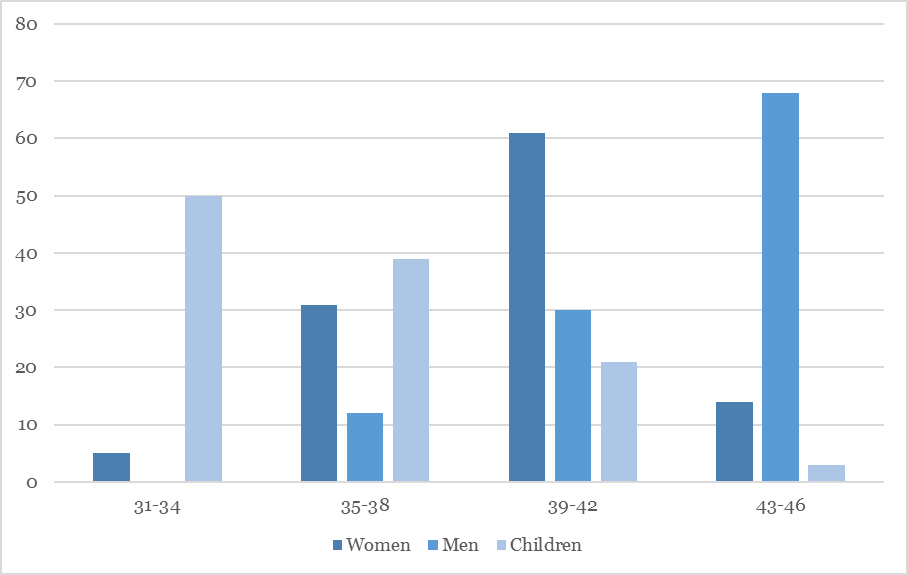
\includegraphics[width=.66\textwidth]{img/example-fig}
% Příponu není potřeba explicitně uvádět, pdflatex automaticky hledá pdf.
% Rozměry také není nutné uvádět.
\caption{Frequency of shoe size in the population of men, women and children (CZSO data, Author’s calculation)}
\label{fig:freq-shoe-size}
\end{figure}

There are several general tips for figures and diagrams.

\begin{itemize}

\item A~figure/diagram should be created in the same size as used in the thesis. 
Decreasing a large diagram leads to having unreadable labels. Increasing a small 
diagram leads to poor graphical quality.

\item The diagram axis shall be properly labelled in the thesis language. 
Missing punctuation is tolerable. If a diagram deals with, e.g., weight and 
height, the labels shall say \emph{Height [cm]} and \emph{Weight [kg]}. If the 
graph includes the function \emph{h(x)}, the axes get a label of \emph{x} and 
\emph{h(x)}. Each axis shall bear a clearly defined scale. 

\item If a two-dimensional diagram marks many points, the author should make 
sure that they do not get mixed. If the number of points is too high, the author 
should decrease the size of the symbols that refer to them or select a lower 
number of points to mark in the diagram. Diagrams with thousands of marked 
points cause problems mainly in electronic documents by increasing the file 
size. 

\item If the thesis is to be printed in black and white, the author should avoid 
using colours. Lines should be distinguished by line type (full, dotted, 
dashed…). Sections should be distinguished by distinct shades of grey or 
hatching. The sense of individual line types or hatched sections shall be 
explained either in the diagram textual legend or in a graphic legend integrated 
into the diagram. 

\item Avoid bitmap figures with a low resolution, especially JPEGs. Compression 
artifacts do not look good on paper. 

\end{itemize}


\section{Source codes}

Algorithms, programme excerpts and descriptions of programme interactions shall 
be distinguished from other text sections. One option is to use package 
\texttt{listings}, which defines a simple \texttt{code} environment in the 
\texttt{makra.tex} file. It can be used to create, for example, the following 
examples.

\begin{code}
> mean(x)
[1] 158.90
> object$mean
[1] 158.90
\end{code}

However, the \texttt{listings} package and its \texttt{lstlisting} environment 
offer an almost inexhaustible number of configuration parameters, eg for 
highlighting the syntax of programming languages (several tens), line numbering, 
etc. Examples:

\begin{itemize}
\item \url{https://en.wikibooks.org/wiki/LaTeX/Source_Code_Listings}
\item \url{https://www.overleaf.com/learn/latex/Code_listing#Using_listings_to_highlight_code}
\end{itemize}


\section{Typesetting of mathematics}

We type the variables in italics (\TeX{} does this in math mode itself, but 
don't forget that in the surrounding text and also turn on math mode). We place 
function names upright. For example:
$\textrm{var} (X) = \textsf{E~} X^2 - \bigl(\textsf{E~} X \bigr)^2$.

Fractions inside a paragraph (e. g. $\frac{5}{7}$ or $\frac{x+y}{2}$) they can 
be too cramped, so it's better to bet simple fractions with a slash: $5/7$, 
$(x+y)/2$.

The possibilities of \LaTeX\ for typesetting mathematics are rich, but they may 
not be sufficient in some specific situations. Therefore, American Mathematical 
Society (AMS) packages can be recommended for use. The \texttt{makra.tex} file 
loads the \texttt{amsmath}, \texttt{amsfonts} and \texttt{amsthm} packages 
by default. To penetrate their possibilities, the following will serve:

\begin{itemize}
\item Math Extension with AMS\LaTeX\ -- \url{http://ptgmedia.pearsoncmg.com/images/0321173856/samplechapter/kopkach15.pdf}
\item \url{https://www.overleaf.com/learn/latex/Aligning_equations_with_amsmath}
\item Math Mode -- \url{http://tex.loria.fr/general/Voss-Mathmode.pdf}
\item More Math into LaTeX -- \url{http://tug.ctan.org/info/Math_into_LaTeX-4/Short_Course.pdf}
\end{itemize}

Example of a numbered formula:
\begin{equation}
\mathbf{b}=(\mathbf{X}^\mathsf{T}\mathbf{X})^{-1}\mathbf{X}^\mathsf{T}\mathbf{y}
\end{equation}

Example of unnumbered formulas with functions and indexes:

$$
d_{ij}=\max_{k=1,2,\dots,n} \{d_{ik}+d_{kj}\},
$$
$$
x_{1,2}=b \pm \sqrt{\ln y}.
$$

An example of a formula as part of one paragraph is given on the example of 
supplier capacities in a mathematical model of a traffic problem, which we take 
into account using constraints:
\begin{equation}
\sum_{j=1}^n x_{ij} \le a_i, \qquad i=1,2,\dots,m\ ,
\end{equation}
\noindent
where expression $a_i$ represents capacity of $i$-th supplier.

When deriving a formula by incremental modification, the individual steps are 
usually listed on separate lines (\verb'align*' environment from the \verb|amsmath| package):

\begin{align*}
 f(x) &= (x+a)(x+b) =\\
      &= x^2 + bx + ax + ab =\\
      &= x^2 + (a+b)x + ab
\end{align*}

Example of column adjustment (\verb|eqnarray*|):
\begin{eqnarray*}
\sum_{i=1}^n x_{ij} =1, && j=1,2,\dots,n,\\
\sum_{j=1}^n x_{ij} =1, && i=1,2,\dots,n,\\
u_i + 1 - M(1 - x_{ij}) \le u_j, && i=2,3,\dots,n,\quad j=1,2,\dots,n,\\
u_i \ge 0,              && i=1,2,\dots,n,\\
x_{ij} \in \{0,1\} && i=1,2,\dots,n,\quad j=1,2,\dots,n,\\
\end{eqnarray*}
\chapter{Work with literature}

The template assumes the use of a bibliographic database for greater flexibility. The use of a bibliographic database is not a necessary condition, it is possible to make do with the standard environment \texttt{thebibliography}. In this case, however, it is necessary to perform interventions on some files, as described below.

\section{Use of bibliographic database}

\begin{enumerate}
\item\textbf{Change the database name}\\
The template assumes a database stored in a file \texttt{bibliography.bib}. If the database is named differently, then it is necessary in the file \texttt{makra.tex} change the value of the  \verb'\bibliography' command parameter.
\item\textbf{Change citation style}\\
By default, citations in the text are given in numerical variant. You can easily switch to using a combination of last name and year by changing the file \texttt{makra.tex}, where the comment character is swapped in the parameters for the package \texttt{biblatex}.
\end{enumerate}


\section{Use of the environment \texttt{thebibliography}}
\begin{enumerate}
\item In the file \texttt{makra.tex} at the beginning delete these lines:
\begin{verbatim}
%%% Nastavení pro použití samostatné bibliografické databáze.
%%% Settings for using a separate bibliographic database.
\usepackage[
   backend=biber
%  ,style=iso-authoryear
  ,style=iso-numeric
  ,sortlocale=cs_CZ
  ,alldates=iso
  ,bibencoding=UTF8
  ,maxnames=2
  ,maxbibnames=99
  %,block=ragged
]{biblatex}
\let\cite\parencite
\renewcommand*{\multinamedelim}{, \addspace}
\renewcommand*{\finalnamedelim}{\addspace a \addspace}

\bibliography{bibliography}
\end{verbatim}
\item In the file \texttt{bibliography.tex} delete the line \verb'\printbibliography' and remove the comment flag in the next section containing the environment \texttt{thebibliography.}
\end{enumerate}


\section{How cite in the text}
\begin{center}
\begin{tabular}{l@{~~$\longrightarrow$~~}l}
\verb|\cite{Cermak2018}|&\cite{Cermak2018}\\
\verb|\cite{Hladik2018,Jasek2018}|&\cite{Hladik2018,Jasek2018}\\
\verb|\cite[chap. 3]{Pecakova2018}|&\cite[kap. 3]{Pecakova2018}\\
\end{tabular}
\end{center}

\chapter{PDF/A format}

Electronic form of final
work must be submitted in PDF/A format level 1a or 2u. They are
PDF profiles that determine which PDF properties are allowed to use
to make the documents suitable for long-term archiving and further automatic
processing. Next we will deal with level 2u, which we bet on \LaTeX{}.

The most important requirements of PDF/A-2u include:

\begin{itemize}

\item All fonts must be built into the document. They are not allowed
links to external fonts.

\item Fonts must contain a ToUnicode table that defines the conversion from encoding
characters used inside a Unicode font. This makes it possible from the document
reliably extract text.

\item The document must contain metadata in XMP format and, if colored,
then also the formal specification of color space.

\end{itemize}

This template uses the {\ tt pdfx} package, which \LaTeX{} can set up
to meet the requirements of PDF/A. Metadata in XMP is generated automatically by
information in the file {\ tt thesis.xmpdata} (you can refer to the generated file
see in {\ tt pdfa.xmpi}).

The correctness of PDF/A can be checked using an online validator: \url{https://www.pdf-online.com/osa/validate.aspx/}.

If the file is not valid, common causes include less use
common fonts (which are inserted only in bitmap format and/or without
unicode tables) and embedding images in PDF, which are standard in themselves
PDF/A do not meet.

This is likely to be the case for images created by many different programs.
In this case, you can try to convert the image to PDF/A using
GhostScript, for example, as follows:

\begin{verbatim}
        gs -q -dNOPAUSE -dBATCH
           -sDEVICE=pdfwrite -dPDFSETTINGS=/prepress
           -sOutputFile=vystup.pdf vstup.pdf
\end{verbatim}

% \include{...}
% \include{...}
{%
\pagestyle{plain}
\chapter*{Závěr}
\addcontentsline{toc}{chapter}{Závěr}

Tématem práce byl \emph{variační autoenkodér a úlohy pozorování v latentním prostoru}.

V první kapitole práce bylo prezentováno široké spektrum možných aplikací modelu variačního autoenkodéru formou stručného shrnutí závěrů dostupných publikací.
Tato kapitola měla za cíl představit čtenáři způsob, jakým lze variační autoenkodér využít, a motivovat ho, aby pokračoval v četbě teoretické části práce.

\textbf{Teoretický úsek výkladu} je považován za \textbf{hlavní přínos této práce}, jelikož postupně staví a detailně interpretuje teoretické aspekty variačního autoenkodéru pomocí následujících kapitol:
\begin{itemize}
    \item \autoref{chap:prereqs} uvádí seznam východisek variačního autoenkodéru, které jsou v oblasti strojového učení stabilně ukotveny.
    \item \autoref{chap:autoencoder} představuje autoenkodér – architekturu modelu strojového učení, na jehož principech staví variační autoenkodér. Byl popsán základní princip fungování autoenkodéru, jeho jednotlivé typy a způsob jejich regularizace. Kapitola je zakončena výkladem o stochastickém autoenkodéru, který slouží jako předchůdce pro uvedení variačního autoenkodéru. 
    \item \autoref{chap:vae} definuje princip fungování variačního autoenkodéru s důrazem na interpretaci jeho teoretických aspektů. Detailně byla rozebrána rovněž účelová funkce variačního autoenkodéru – konkrétně její dva prvky: KL divergence a chyba rekonstrukce, včetně role, kterou v trénovacím procesu modelu zastávají. Závěrem kapitoly byl krátce shrnut aktuální stav poznání variačního autoenkodéru, jeho existující rozšíření a omezení.
\end{itemize}

V tomto jde práce nad rámec monografie autorů variačního autoenkodéru \textcite{Kingma2019} a propojuje variační autoenkodér s architekturou různých typů autoenkodéru a dalších definic z oblasti strojového učení (autoři monografie předpokládají znalost této látky a tak ji ve své monografii neuvádí).

Následně byl na základě zavedené teorie prakticky implementován \textbf{ilustrační} model variačního autoenkodéru pro generativní úlohu obrazových dat MNIST.
Latentní prostor naučeného modelu byl formou vizualizací analyzován a interpretován. Závěrem kapitoly jsou diskutovány možnosti evaluace generativních modelů variačního autoenkodéru.

Výsledkem práce je \textbf{ucelený} výklad o variačním autoenkodéru, který na jednom místě shrnul možnosti jeho multidisciplinárních aplikací, definoval a interpretoval jeho teoretické aspekty a prakticky implementoval ilustrační model variačního autoenkodéru pro generativní úlohu obrazových dat MNIST.
K implementovanému modelu a jeho vizualizacím jsou rovněž přiloženy kompletní zdrojové kódy pro snadnou replikaci.
}

%%% Seznam použité literatury
%%% Bibliography
%% This applies if a separate bibliographic database is used
\printbibliography[title={\bibname},heading={bibintoc}]

%% This is true when using thebibliography environment
%% The following can be recommended for compiling citation data:
%%     https://knihovna.vse.cz/citace/priklady/
%%     https://www.citace.com/
%\openright
%\phantomsection
%\addcontentsline{toc}{chapter}{\bibname}
%\begin{thebibliography}{99}
%\bibitem{Cermak2018}ČERMÁK, Radim, SMUTNÝ, Zdeněk. A Framework for Cultural Localization of Websites and for Improving Their Commercial Utilization. In:  \emph{Global Observations of the Influence of Culture on Consumer Buying Behavior} [online]. Hershey~: IGI Global, 2018, s. 206--232. ISBN 978-1-5225-2727-5. DOI: 10.4018/978-1-5225-2727-5.
%
%\bibitem{Hladik2018}HLADÍK, Milan, ČERNÝ, Michal. The Shape of the Optimal Value of a Fuzzy Linear Programming Problem. In: \emph{Fuzzy Logic in Intelligent System Design} [online]. Cancum, 16.10.2017 -- 18.10.2017. Cham~: Springer, 2018, s. 281--286. Advances in Intelligent Systems and Computing 648. ISBN 978-3-319-67136-9. DOI: 10.1007/978-3-319-67137-6\_31.
%
%\bibitem{Jasek2018}JAŠEK, Pavel, VRANÁ, Lenka, ŠPERKOVÁ, Lucie, SMUTNÝ, Zdeněk, KOBULSKÝ, Marek. Modeling and Application of Customer Lifetime Value in Online Retail. \emph{Informatics} [online]. 2018, roč. 5, č. 1. 22 s. eISSN 2227-9709. DOI: 10.3390/informatics5010002. Dostupné také z: \url{http://www.mdpi.com/2227-9709/5/1/2/pdf}.
%
%\bibitem{Pecakova2018}PECÁKOVÁ, Iva. \emph{Statistika v terénních průzkumech}. 3. přeprac. vyd. Praha~: Professional Publishing, 2018. 254 s. ISBN 978-80-88260-10-3.
%\end{thebibliography}


%%% Přílohy k práci, existují-li. Každá příloha musí být alespoň jednou
%%% odkazována z vlastního textu práce. Přílohy se číslují.
%%% Attachments to thesis, if any. Each attachment must be referenced at 
%%% least once in your own text. The appendices are numbered.
\part*{\Prilohy\thispagestyle{empty}}
\appendix
\chapter{Zdrojové kódy modelů}
\label{app:vae_model_source_code}

Přiložený soubor \emph{\lstinline|bachelor-thesis-source-code.zip|} obsahuje:

\begin{itemize}
    \item \emph{\lstinline|vae_mnist_train.py|}
    \item \emph{\lstinline|vae_mnist_train.pynb|}
    \item \emph{save}
    \item \emph{model}
    \item \emph{loaders}
\end{itemize}

Pro spuštění trénovací fáze a vizualizací jsou potřeba následující programy a balíčky:
\begin{itemize}
    \item Python 3.12.
    \item TensorFlow 2.12.0.
    \item Matplotlib 3.7.1.
    \item Numpy 1.24.0
    \item Jupyter notebook 6.5.4.
\end{itemize}

Trénovací fáze se spustí souborem \lstinline|vae_mnist_train.py|, vizualizace pak \lstinline|vae_mnist_train.pynb|.
\begin{landscape}
    \chapter{Vývoj latentního prostoru naučeného modelu skrze různý počet epoch}
    \label{app:latent_space_development}

    \begin{figure}[H]
        \centering
        \subfloat[\centering label 1]{{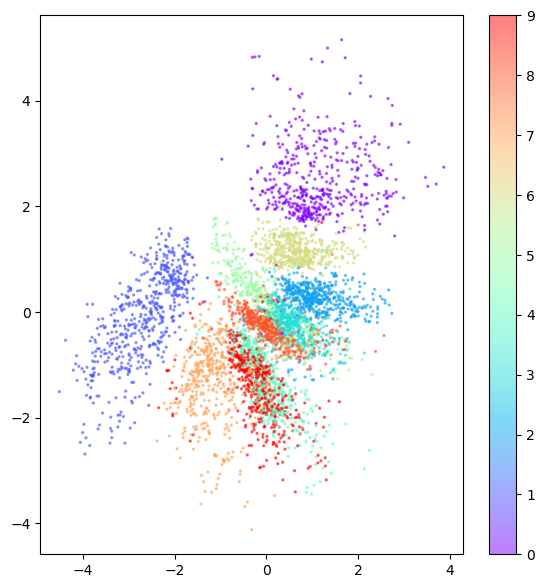
\includegraphics[width=0.50\textwidth]{figures/latent_space_200_epochs.png} }}%
        \subfloat[\centering label 2]{{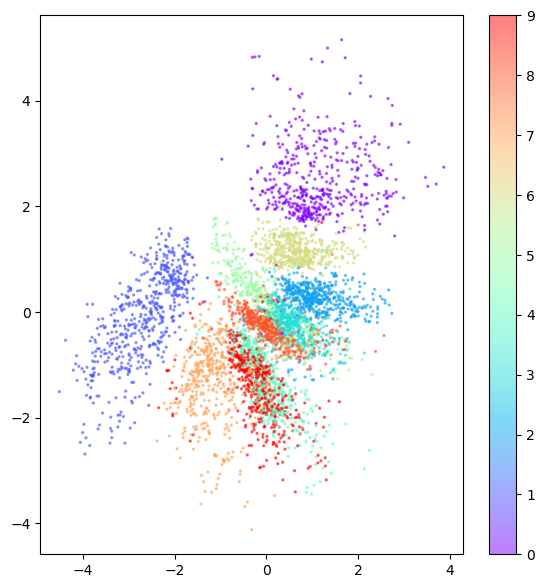
\includegraphics[width=0.50\textheight]{figures/latent_space_200_epochs.png} }}%
        \subfloat[\centering label 3]{{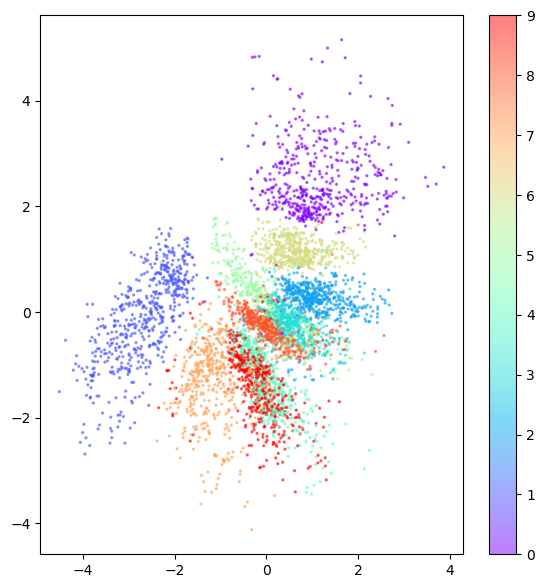
\includegraphics[width=0.50\textheight]{figures/latent_space_200_epochs.png} }}%
        \caption{2 Figures side by side}%
        \label{fig:example}%
    \end{figure}

\end{landscape}
% \include{...}
% \include{...}

\end{document}
